\documentclass{article}


% if you need to pass options to natbib, use, e.g.:
%     \PassOptionsToPackage{numbers, compress}{natbib}
% before loading neurips_2023

% ready for submission
\usepackage[final]{neurips_2023}

% to avoid loading the natbib package, add option nonatbib:
%    \usepackage[nonatbib]{neurips_2023}


\usepackage[utf8]{inputenc} % allow utf-8 input
\usepackage[T1]{fontenc}    % use 8-bit T1 fonts
\usepackage{hyperref}       % hyperlinks
\usepackage{url}            % simple URL typesetting
\usepackage{booktabs}       % professional-quality tables
\usepackage{amsfonts}       % blackboard math symbols
\usepackage{nicefrac}       % compact symbols for 1/2, etc.
\usepackage{microtype}      % microtypography
\usepackage{xcolor}         % colors
\usepackage{graphicx}       % addtional package for show figures


\begin{document}


\maketitle

\section{Experiments}

\subsection{Linear SVM}
\begin{itemize}
  \item \textbf{Hyperparameter:} Regularization coefficient $C \in \{0.01, 0.1, 1, 10, 100\}$.
  \item \textbf{Performance Curve:} Training F1 $\approx0.7787$, Validation F1 $\approx0.7747$ remain stable across $C$.
  \item \textbf{Over- vs.\ Under-fitting:} Train F1 $\approx$ Val F1, both well below 1.0 $\rightarrow$ slight under-fitting; no over-fitting observed.
  \item \textbf{Conclusion:} $C=1$ offers a good trade-off; further tuning yields no significant gain.
\end{itemize}

\subsection{Decision Tree}
\begin{itemize}
  \item \textbf{Hyperparameter:} Maximum depth $\text{max\_depth} \in \{5, 10, 15, 20, \text{None}\}$.
  \item \textbf{Performance Curve:}
    \begin{itemize}
      \item $\text{depth}=5$: Train/Val F1 $\approx0.65$ (under-fitting).
      \item $\text{depth}=10$: Best validation F1 $\approx0.674$ (Train $\approx0.807$).
      \item $\text{depth}>10$: Train F1 increases, Val F1 decreases (over-fitting).
    \end{itemize}
  \item \textbf{Over- vs.\ Under-fitting:} Depth $<10$ under-fits; depth $>10$ over-fits.
  \item \textbf{Conclusion:} Optimal depth $=10$; deeper trees memorize noise and degrade generalization.
\end{itemize}

\subsection{SGDClassifier (Logistic Regression)}
\begin{itemize}
  \item \textbf{Hyperparameter:} L2 regularization strength $\alpha \in \{10^{-6},10^{-5},10^{-4},10^{-3},10^{-2},10^{-1}\}$.
  \item \textbf{Performance Curve:}
    \begin{itemize}
      \item $\alpha=10^{-5}$: Best Train F1 $\approx0.7483$, Val F1 $\approx0.7480$.
      \item $\alpha\ge10^{-4}$: Both F1 scores drop (under-fitting).
      \item $\alpha=10^{-6}$: Train F1 $>$ Val F1 (slight over-fitting).
    \end{itemize}
  \item \textbf{Over- vs.\ Under-fitting:} \(\alpha\gg10^{-5}\) under-fits; \(\alpha\ll10^{-5}\) over-fits.
  \item \textbf{Conclusion:} $\alpha=10^{-5}$ balances bias and variance well.
\end{itemize}

\begin{figure}[h]
  \centering
  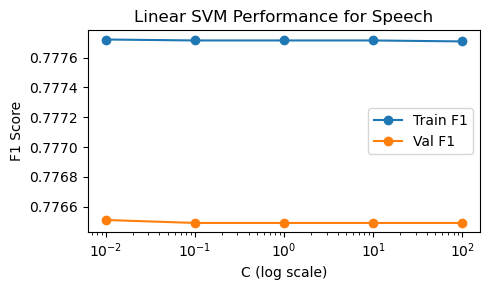
\includegraphics[width=0.3\linewidth]{tang/svm.png}
  \hfill
  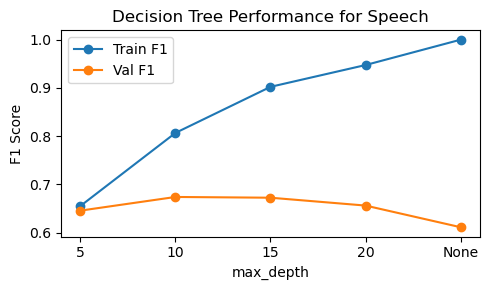
\includegraphics[width=0.3\linewidth]{tang/dt.png}
  \hfill
  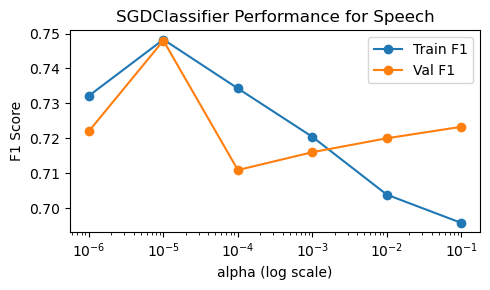
\includegraphics[width=0.3\linewidth]{tang/sgd.png}
  \caption{Performance curves for Linear SVM (left), Decision Tree (middle), and SGDClassifier (right).}
  \label{fig:hp_curves}
\end{figure}

\subsection{Model Comparison}
\begin{table}[h]
\centering
\begin{tabular}{lccc}
\toprule
\textbf{Model} & \textbf{Best Hyperparameter} & \textbf{Validation F1} & \textbf{Avg Training Speed} \\
\midrule
Linear SVM     & $C=1$                        & 0.7748                & 44 s/class             \\
SGDClassifier  & $\alpha=10^{-5}$             & 0.7480                & 5–90 s/class            \\
Decision Tree  & max\_depth=10                & 0.6741                & 438 s/class             \\
\bottomrule
\end{tabular}
\caption{Comparison of the three classifiers on the validation set.}
\end{table}

\subsection{Final Model Performance}
The selected model (Linear SVM with $C=1$) was evaluated on the held-out test set using six features.
The overall Macro-F1 score across 58 classes is \textbf{0.5381}, reflecting average performance on frequent and rare classes.





\end{document}